% Chapter 4

\chapter{SYSTEM DESIGN} % All Chapter headings in ALL CAPS

\section{System Architecture}

The block diagram for the entire system is shown in figure 4.1. The
system aims to secure the insurance data by storing it in the blockchain. Since the insurance data is very large in size, we have restricted our system to the treatments that falls in the policies alone. Initially the organization and the peers for each organization is created in the blockchain network using HyperLedger Fabric. Each organization will have a certifying authority that endorses the peer that it belongs to its organization. The Docker is used to virtualize the environment to allow multiple peers to work on same system. The chaincode is the smart contract that automatically executes when an transaction takes place. The data in each block are encrypted using Private Key Encryption and hashed using SHA256. 
\newline
\newline
\newline
\newline
\newline
\newline
\newline
\newline
\newline



\begin{figure}[htb!]
  \centering
 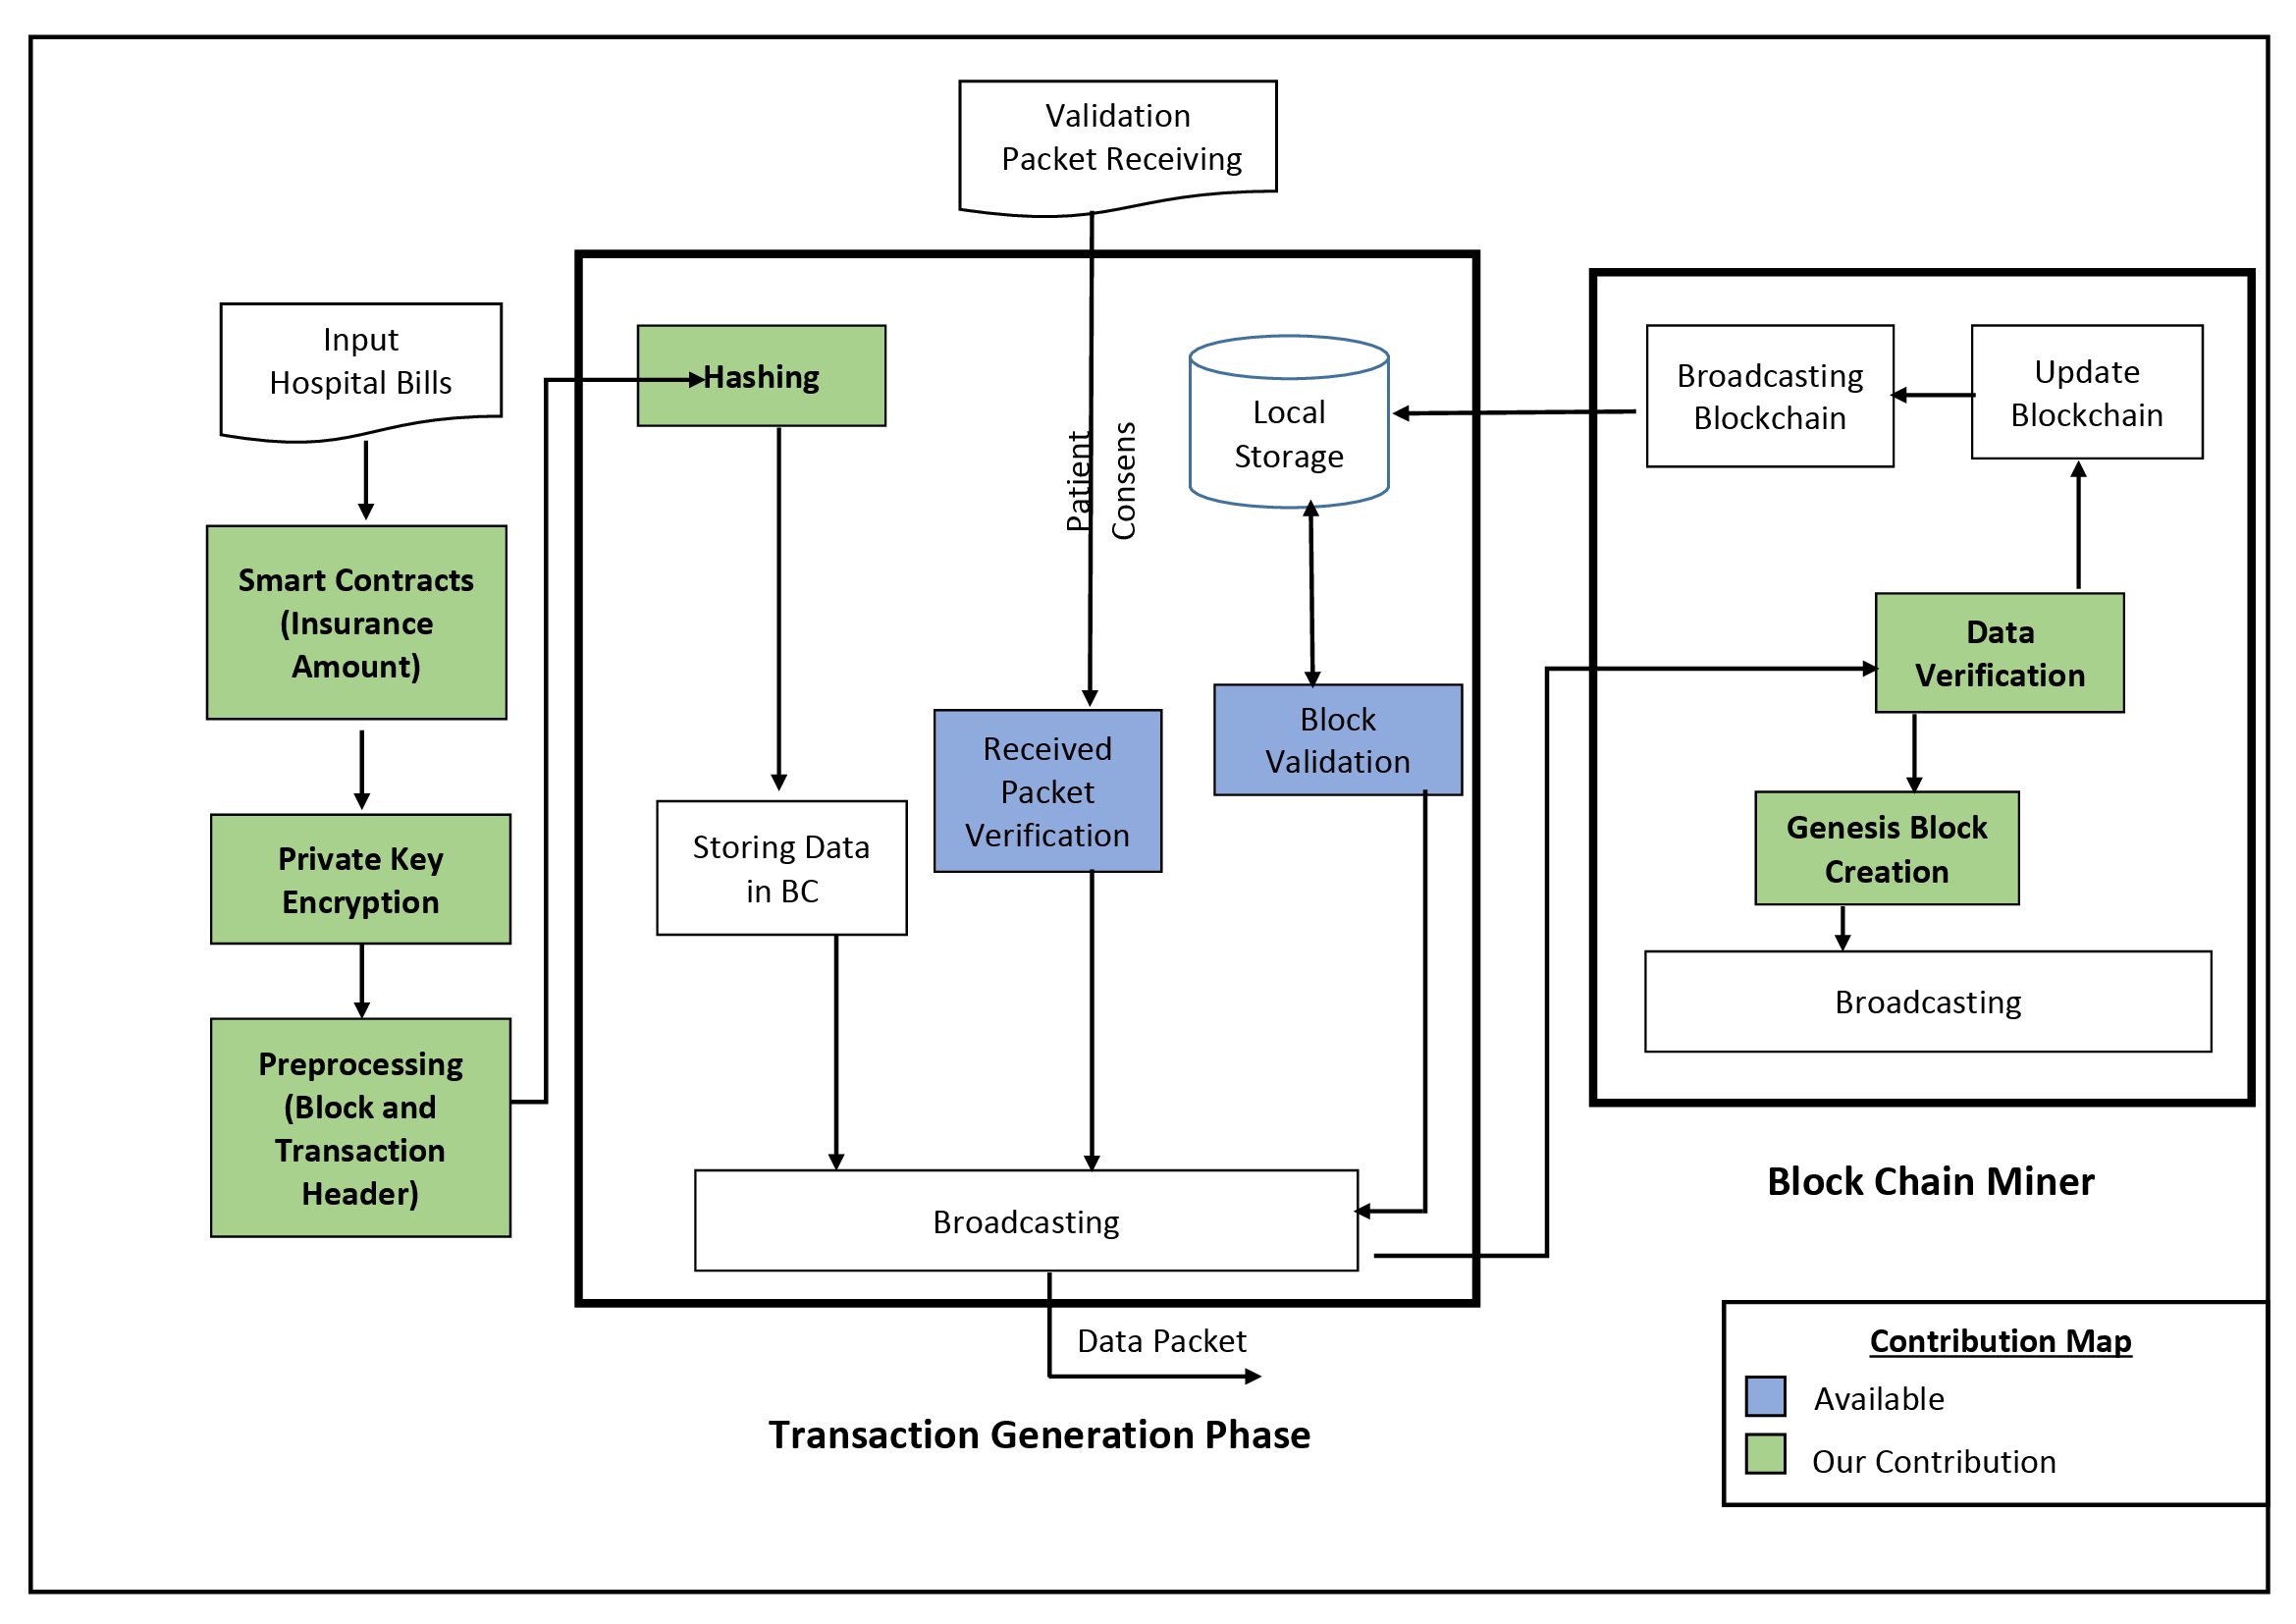
\includegraphics[width = 15cm, height = 12cm, angle=90, scale=1.3]{Figures/Block-Diagram.png}
  \caption{Block Diagram}
  \label{StH}	
\end{figure}

\section{Module Design}
\lipsum[]
Our architecture has three phases.
\begin{itemize}
    \item Pre-processing phase has three modules.
    \begin{enumerate}
        \item Smart Contracts
\item Private Key Encryption
\item Preprocessing
    \end{enumerate}
    \item Transaction Generation Phase has four modules.
    \begin{enumerate}
        \item Hashing
\item Received Packet Verification
\item Block Validation
\item Broadcasting
    \end{enumerate}
    \item Blockchain Miner has three modules.
    \begin{enumerate}
        \item Data Verification
\item Genesis Block Creation
\item Broadcasting Blockchain
    \end{enumerate}
    \end{itemize}
\section{Preprocessing Phase}
In this phase we have implemented smart contracts to decide whether to initiate the transaction or not. We have also encrypted the data using RSA algorithm to restrict the access.
\subsection{Smart Contracts}
It takes the Bill ID and Bill amount as input. Smart Contracts automatically claims the patient bill amount whose insurance amount must be less than the insurance limit. And if the insurance amount is less than or equal to the insurance limit the data is sent to the encrypted phase if not it is discarded.
\subsection{Private Key Encryption}
It takes the patient treatment details as the input and encrypts the data using RSA Algorithms and produces the encrypted data.
\subsection{Preprocessing}
It takes the encrypted data as input and checks all the necessary data to instantiate a claim that has been uploaded or not and produces the block containing the block header and transaction header.
\section{Transaction Generation Phase}
Once the treatment has been made then patient’s details should be stored in blockchain. This phase contains hashing the patient details, treatment details and verification processes. Every transaction begins in this phase.
\subsection{Hashing}
It takes the block containing the block header and transaction header as the input and hashes the data in the block using SHA-256 algorithm.
\subsection{Received Packet Verification}
In blockchain every transaction has to be verified by other peers in a network to take appropriate decision. The following steps has to be done in this module.
\subsection{Block Validation}
This module is available in every peer of the blockchain network. The peers in the network obtains the newly mined block from the miner. They check the validity of the block. If valid they update their blockchain else discards the new block. Procedure for the block validation is given below.
\section{Blockchain Miner}
In this phase new block will be generated by the miner by solving proof of work and updates the blockchain. This module contains genesis block creation, data Verification, broadcasting blockchain.
\subsection{Data Verification}
This module finds a hash below a targeted hash value (PoW). We have four types of algorithms for consensus in blockchain. Consensus is the only algorithm we can use. Four types of algorithms are:
\begin{itemize}
    \item Practical Byzantine Fault Tolerance Algorithm
\item Proof-of-work
\item Proof-of-Stake
\item Delegated Proof-of-Stake
\end{itemize}
\subsection{Consensus Algorithm}
The proof of work is a computational client puzzle where computation power is needed to solve the puzzle and the nodes who solve the puzzle first will add the block to blockchain and will get a reward in mining network. Once a block is completed, it will be broadcasted to all the mining nodes and all of them start to mine. The miner node who solves that first will add that block to block chain.
\subsection{Genesis Block Creation}
In this module, the genesis block for bootstrapping the blockchain application is created using configtxgen tool which is an inbuilt tool with Hyper ledger. This tool takes an input file configtx.yaml and outputs the binary file which should be used when creating initial setup for blockchain.
\subsection{Broadcasting Blockchain}
This module broadcasts the newly created block to other peers in the network.